\documentclass{beamer}
\usepackage[T1]{fontenc}
\usepackage{lmodern}
\usepackage{latexsym,amsmath,amsthm,xcolor,multicol,booktabs,calligra,bookmark}
\usepackage{tikz,physics,subcaption}
\usepackage[compat=1.1.0]{tikz-feynman}
\usepackage{graphicx,pstricks,listings,stackengine}
\usepackage{hyperref}
\usepackage{physics}

\author{JiaHao Miao}
\title{\textbf{Computational Physics Laboratory:\\
       Tree Level Gluon Amplitudes in Mathematica}}
\institute{
    Università degli Studi di Milano\\
    Dipartimento di Fisica "Aldo Pontremoli"
}

\date{\today}
\usepackage{style/Presentation}

% defs
\def\cmd#1{\texttt{\color{red}\footnotesize $\backslash$#1}}
\def\env#1{\texttt{\color{blue}\footnotesize #1}}
\definecolor{deepblue}{rgb}{0,0,0.5}
\definecolor{deepred}{rgb}{0.6,0,0}
\definecolor{deepgreen}{rgb}{0,0.5,0}
\definecolor{halfgray}{gray}{0.55}

\lstset{
  basicstyle=\ttfamily\small,
  breaklines=true,
  showstringspaces=false,
  commentstyle=\color{gray},
  keywordstyle=\color{blue},
  stringstyle=\color{purple},
  numberstyle=\tiny\color{gray},
  numbers=left,
  stepnumber=1,
  numbersep=5pt,
  backgroundcolor=\color{gray!10},
  frame=single,
  framesep=5pt,
  rulesep=0pt,
  xleftmargin=5pt,
  xrightmargin=5pt
}

\renewcommand{\lstlistingname}{Mathematica} % Change "Listing" to "Code"

\begin{document}

\begin{frame}
    \titlepage
\end{frame}

% Table of Contents slide
% \frame{\tableofcontents[sectionstyle=show,subsectionstyle=show/shaded/hide,subsubsectionstyle=show/shaded/hide]}


\section*{Problem}
\begin{frame}{Tree Level Gluon Scattering Amplitudes}
    \begin{itemize}
        \item How: Well-established theoretical framework using Feynman diagrams.
        \item In Practice:
        \begin{itemize}
            \item Rapidly increasing number of diagrams as the number of external legs increases.   
            \item Proliferating of algebraic expressions.
            \item Lorentz indices and color indices complicate the calculations.
        \end{itemize}
        \item Number of tree-level diagrams for $n+1$ gluons grows more than factorially:
        $$ \order{\left(\frac{9\sqrt{3}+12}{11}\right)^{n}\frac{n!}{n^{3/2}}} $$ 
    \end{itemize}
\end{frame}

\begin{frame}[fragile]{Feynman Diagrams in Mathematica}

    Represent each diagram as a list of pairs and use Mathematica's symbolic capabilities to manipulate these lists.
    \begin{figure}[ht]
        \centering
        \begin{subfigure}[b]{0.48\textwidth}
            \centering
            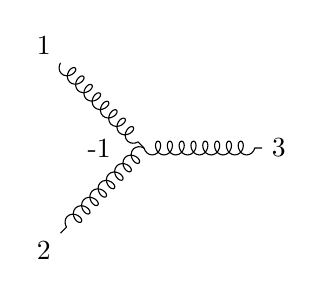
\begin{tikzpicture}
                \begin{feynman}
                    \vertex [label={[xshift=-3mm]left:{-1}}](a);
                    \vertex [above left =of a] (i1) {$1$};
                    \vertex [below left =of a] (i2) {$2$};
                    \vertex [right =of a] (f1) {$3$};

                    \diagram* {
                        (i1) -- [gluon] (a) -- [gluon] (i2);
                        (a) -- [gluon] (f1);
                    };
                \end{feynman}
            \end{tikzpicture}
            \caption*{ \{\{1,-1\},\{2,-1\},\{3,-1\}\}}
        \end{subfigure}
        \hfill
        \begin{subfigure}[b]{0.48\textwidth}
            \centering
            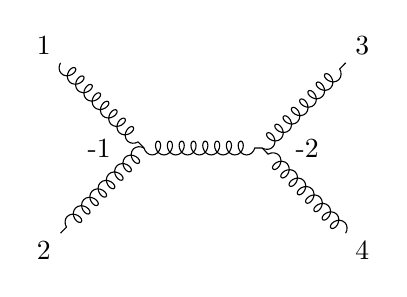
\begin{tikzpicture}
                \begin{feynman}
                    \vertex [label={[xshift=-3mm]left:{-1}}](a);
                    \vertex [above left =of a] (i1) {$1$};
                    \vertex [below left =of a] (i2) {$2$};
                    \vertex [label={[xshift=+3mm]right:{-2}}](b) [right=of a];
                    \vertex [above right =of b] (f1) {$3$};
                    \vertex [below right =of b] (f2) {$4$};

                    \diagram* {
                        (i1) -- [gluon] (a) -- [gluon] (i2);
                        (a) -- [gluon] (b);
                        (f2) -- [gluon] (b)--[gluon] (f1);
                    };
                \end{feynman}
            \end{tikzpicture}
            \caption*{ \{\{1,-1\},\{2,-1\},\{-1,-2\},\{3,-2\},\{4,-2\}\}}
        \end{subfigure}
    \end{figure}
\end{frame}

\begin{frame}{Number of Diagrams}
    \begin{table}[htbp]\centering
        \begin{tabular}{c c c c }
            \hline
            \textbf{n} & \textbf{Diagrams} & \textbf{only 3-point} & \textbf{with 4-point} \\
            \hline
            4 & 4 & 3 & 1 \\
            5 & 25 & 15 & 10 \\
            6 & 220 & 105 & 115 \\
            7 & 2485 & 945 & 1540 \\
            8 & 34300 & 10395 & 23905 \\
            9 & 559405 & 135135 & 424270 \\
            10 & 10525900 & 2027025 & 8498875 \\
            \hline    
        \end{tabular}
    \end{table}
    \begin{itemize}
        \item Number of diagrams with only 3-point vertices: $(2n-5)!!$
        \item Diagrams with only 3-point vertices brings unique color structures.
        \end{itemize}
\end{frame}

\begin{frame}{Memory and Time Complexity}
    \centering
    \begin{table}
        \caption*{$\mathcal{M} = \sum \text{diagrams} $}
        \scriptsize
        \resizebox{\textwidth}{!}{
            
            \begin{tabular}{|c|c|c|c|c|c|}
                \hline
                \textbf{n} & \textbf{Diagrams} & \textbf{Diagrams (s)} & \textbf{Diagrams (MB)} & \textbf{Amplitude (s)} & \textbf{Amplitude (MB)} \\
                \hline
                4 & 4 & 0.0011 & 0.01 & 0.004 & 0.096 \\ 
                5 & 25 & 0.0100 & 0.12 & 0.051 & 2.87 \\ 
                6 & 220 & 0.1153 & 1.51 & 6.503 & 104.52 \\ 
                7 & 2485 & 1.5998 & 22.99 & 1112.738 & 4430.25 \\ 
                8 & 34300 & 27.5766 & 404.70 & TBD & TBD \\ 
                \hline
            \end{tabular}
        }
    \end{table}
\end{frame}

\section{Benchmarks}


\begin{frame}{Ward Identities}
  \centering 
    \begin{figure}
          \includegraphics[width=\textwidth, keepaspectratio]{figures/ward.png}
    \end{figure}
\end{frame}

\begin{frame}{Modulus Squared}
  \centering 
    \begin{figure}
          \includegraphics[width=\textwidth, keepaspectratio]{figures/Modulus.png}
    \end{figure}
\end{frame}

\end{document}